\begin{figure}[h!]
\textbf{Tema d'Esame di Febbraio 2017}\\ \\
Sapendo che la resistenza $R8$ è attraversata da una corrente $i_8 = 0.20 A$, si calcoli la corrente che attraversa $R3$. Si considerino le seguenti resistenze $R8 = 10 \Omega, R1 = R2 = R3 = 5.0 \Omega , R4 = 12 \Omega , R5 = 15 \Omega $.
	\begin{center}
		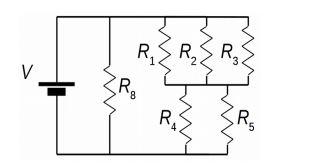
\includegraphics[scale=1.1]{ES5/FEB052017.jpg}
	\end{center}
	\noindent\fbox{
		\parbox{\textwidth}{
			\null\hfill \textbf{Soluzione:} $I_3 = 0.08A$\\
			\textbf{Procedimento: } \\
			Semplificazione delle Resistenze:\\
			$R_{123}=\frac{1}{\frac{1}{R_1}+\frac{1}{R_2}+\frac{1}{R_3}}=\frac{1}{\frac{1}{5\Omega}+\frac{1}{5\Omega}+\frac{1}{5\Omega}}=1.67\Omega$\\ \\ 
			$R_{45}=\frac{R_4\cdot R_5}{R_4 + R_5}=\frac{12\Omega\cdot 15\Omega}{12\Omega + 15\Omega}=6.67\Omega$\\
			$R_{12345}=R_{123}+R_{45}=6.67\Omega+1.67\Omega=8.34\Omega$\\
			Ricordando che la tensione in parallelo non cambia, così come non cambia la corrente in serie:\\
			$V_{tot}=V_{12345}=V_8=R_8\cdot I_8=10\Omega\cdot 0.2A=2V$\\
			$I_{12345}=I_{123}=I_{45}=\frac{V}{R_{12345}}=\frac{2V}{8.34\Omega}=0.24A$\\
			$V_{123}=R_{123}\cdot I_{12345}=1.67\Omega\cdot 0.24A=0.40V$\\
			$I_3=\frac{V_{123}}{R_3}=\frac{0.40V}{5\Omega}=0.08A$
		}
	}	
	
\end{figure}

\begin{figure}[h!]
\textbf{Tema d'Esame di Giugno 2017}\\ \\
 Si determini il valore della resistenza $R_x$ del circuito mostrato nella figura sotto a sinistra. La differenza di potenziale fornita dalla batteria è $3 V$, la corrente $i_3$ che scorre nella resistenza $R_3$ è pari a $0.1 A$ ed i valori delle altre resistenze nel circuito
sono $R1 = R2 = 5 \Omega ,R3 = R4 = 10 \Omega$.
	\begin{center}
		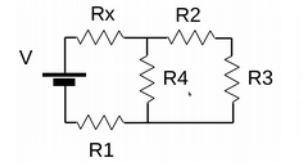
\includegraphics[scale=1.1]{ES5/GIU052017.jpg}
	\end{center}
	\noindent\fbox{
		\parbox{\textwidth}{
			\null\hfill \textbf{Soluzione:} $R_x = 1\Omega$\\
			\textbf{Procedimento: } \\
			Ricordando che la tensione in parallelo non cambia, così come non cambia la corrente in serie proseguiamo semplificando le resistenze e aggiornando man mano corrente e tensione:\\
			
			$R_{23}=R_2 + R_3=5\Omega + 10\Omega=15\Omega$\\
			$I_3=I_2=I_{23}=0.1A$\\
			$V_{23}=V_{234}=V_4=R_{23} \cdot I_{23}=15\Omega \cdot 0.1A=1.5V$\\
			$I_{234}=\frac{V_{234}}{R_{234}}=\frac{1.5V}{6\Omega}=0.25A$\\
			$V_1=R_1\cdot I_{234}=5\Omega \cdot 0.25A=1.25V$\\
			$V_x=V_{tot}- V_1 - V_{234}=3V - 1.25V -1.5V=0.25V$\\
			$R_x=\frac{V_x}{I_{234}}=\frac{0.25V}{0.25A}=1\Omega$
		}
	}	
\end{figure}

\begin{figure}[h!]
\textbf{Tema d'Esame di Settembre 2017}\\ \\
Trovare le correnti $i_1, i_2 , i_3$ nei tre rami del circuito qui sotto.
$R1 = 4.0 \Omega, R2 = 6.0 \Omega, R3 = 3.0 \Omega$ ed $ E 1 = 1.5 V,  E 2 = 3.0 V$.
	\begin{center}
		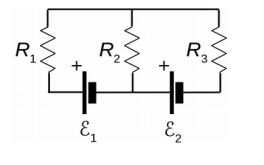
\includegraphics[scale=1.1]{ES5/SET052017.jpg}
	\end{center}
	\noindent\fbox{
		\parbox{\textwidth}{
			\null\hfill \textbf{Soluzione:} $R_x = 1\Omega$\\
			\textbf{Procedimento: } \\
			In questa tipologia di esercizio si deve impostare il sistema per poi trovare le rispettive correnti, per farlo bisogno stabilire arbitrariamente il verso della corrente di ogni maglia.\\
			 Nel nostro caso supporremo che la corrente viaggi in senso orario in entrambe le maglie.\\

			\systeme*{
				I_1=I_2 +I_3,
				\varepsilon_1= R_1\cdot I_1 + R_2\cdot I_2,
				\varepsilon_2= -R_2\cdot I_2 + R_3\cdot I_3
			}
			\\ \\
			Risolvendo il sistema si otterranno i valori delle correnti.\\ \\
			\systeme*{
				I_1=I_2 +I_3,
				1.5= 4\cdot I_1 + 6\cdot I_2,
				3= -6\cdot I_2 + 3\cdot I_3
			}
			\hspace{1.5cm} = \hspace{1.5cm}
			\systeme*{
				I_1=I_2 +I_3,
				1.5= 4\cdot I_2 + 4\cdot I_3 + 6\cdot I_2,
				3= -6\cdot I_2 + 3\cdot I_3
			}\\ \\
			\systeme*{
				I_1=I_2 +I_3,
				1.5= 10\cdot I_2 + 4\cdot I_3,
				I_3=\frac{3V +6\cdot I_2}{3}
			}
			\hspace{1.5cm} = \hspace{1.5cm}
			\systeme*{
				I_1=I_2 +I_3,
				1.5= 10\cdot I_2 + 4\cdot (1 +2\cdot I_2),
				3= -6\cdot I_2 + 3\cdot I_3
			}\\ \\
			\systeme*{
				I_1=I_2 +I_3,
				I_2= -0.139,
				I_3= 1 +2\cdot I_2
			}
			\hspace{1.5cm} = \hspace{1.5cm}
			\systeme*{
				I_1=-0.139 +I_3,
				I_2= -0.139,
				I_3= 0.722
			}\\ \\
			\systeme*{
				I_1= 0.583A,
				I_2= -0.139A,
				I_3= 0.722A
			}\\ \\
		}
	}	
	
\end{figure}